\section{OS Concepts}

\paragraph{OS Invocation}
\begin{items}
	\item OS Kernel does \textbf{not} always run in background!
	\item Occasions invoking kernel, switching to kernel mode:
	\begin{enumeration}
		\item \textbf{System calls}: User-Mode processes require higher privileges
		\item \textbf{Interrupts}: CPU-external device sends signal
		\item \textbf{Exceptions}: CPU signals unexpected condition
	\end{enumeration}
\end{items}

\paragraph{System Calls --- Motivation}
\begin{items}
	\item \textbf{Problem}: protect processes from one another
	\item \textbf{Idea}: Restrict processes by running them in user-mode
	\item \textbf{\( \leadsto \) Problem}: now processes cannot manage hardware,... \\*
		who can switch between processes? \\*
		who decides if process may open certain file?
	\item \textbf{\( \leadsto \) Idea}: OS provides \textbf{services} to apps \\*
		app calls system if service is needed (\textbf{syscall}) \\*
		OS checks if app is allowed to perform action \\*
		if app may perform action and hasn't exceeded quota, \\* \phantom{x} OS performs action in behalf of app in kernel mode
\end{items}

\paragraph{System Calls --- Examples}
\begin{items}
	\item \code{fd = open(file, how,...)} -- open file for read/write/both
	\item documented e.g. in \code{man 2 write}
	\item overview in \code{man 2 syscalls}
\end{items}

\paragraph{System Calls vs. APIs}
\begin{items}
	\item \textbf{syscalls}: interface between apps and OS services, limited number of well-defined entry points to kernel
	\item \textbf{APIs}: often used by programmers to make syscalls \\*
		e.g. \code{printf} library call uses \code{write} syscall
	\item common APIs: Win32, POSIX, C API
\end{items}

\paragraph{System Calls --- Implementation}
\begin{items}
	\item \emph{trap instruction}: single syscall interface (entry point) to kernel \\*
		switches CPU to kernel mode, enters kernel in same, predefined \\* \phantom{x} way for all syscalls \\*
		system call dispatches then acts as syscall multiplexer
	\item syscalls identified by number passed to trap instruction \\*
		\textbf{syscall table} maps syscall numbers to kernel functions \\*
		dispatcher decides where to jump based on number and table \\*
		programs (e.g. \code{stdlib}) have syscall number compiled in! \\*
		\( \leadsto \) never reuse old numbers in future kernel versions
\end{items}

\paragraph{Interrupts}
\begin{items}
	\item devices use interrupts to signal predefined conditions to OS \\*
		reminder: device has "`interrupt line"' to CPU \\*
		e.g. device controller informs CPU that operation is finished
	\item \textbf{programmable interrupt controller} manages interrupts \\*
		interrupts can be \textbf{masked} \\*
		masked interrupts: queued, delivered when interrupt unmasked \\*
		queue has finite length \( \leadsto \) interrupts can get lost
	\item notable interrupt examples:
	\begin{enumeration}
		\item \emph{timer-interrupt}: periodically interrupts processes, switches to kernel \( \leadsto \) can then switch to different processes for fairness
		\item \emph{network interface card} interrupts CPU when packet was received \( \leadsto \) can deliver packet to process and free NIC buffer
	\end{enumeration}
	\item when interrupted, CPU
	\begin{enumeration}
		\item looks up \textbf{interrupt vector} (= table pinned in memory, contains addresses of all service routines)
		\item transfers control to respective \textbf{interrupt service routine} in OS that handles interrupt
	\end{enumeration}
	\item interrupt service routine must first save interrupted process's state (instruction pointer, stack pointer, status word)
\end{items}

\paragraph{Exceptions}
\begin{items}
	\item sometimes unusual condition makes it impossible for CPU to continue processing
	\item \( \leadsto \) \textbf{Exception} generated within CPU:
	\begin{enumeration}
		\item CPU interrupts program, gives kernel control
		\item kernel determines reason for exception
		\item if kernel can resolve problem \( \leadsto \) does so, continues \textbf{faulting instruction}
		\item kills process if not
	\end{enumeration}
	\item Difference to Interrupts: interrupts can happen in any context, exceptions always occur asynchronous and in process context
\end{items}

\paragraph{OS Concepts --- Physical Memory}
\begin{items}
	\item up to early 60s: \\* 
		- programs loaded and run directly in \emph{physical memory}
		\\*
		- program too large \( \to \) partitioned manually into \emph{overlays}
		\\*
		- OS then swaps overlays between disk and memory
		\\*
		- different jobs could observe/modify each other
\end{items}

\paragraph{OS Concepts --- Address Spaces}
\begin{items}
	\item bad programs/people need to be isolated
	\item \textbf{Idea}: give every job the illusion of having all memory to itself
		\\*
		every job has own \emph{address space}, can't name addresses of others
		\\*
		jobs always and only use virtual addresses
\end{items}

\paragraph{Virtual Memory --- indirect addressing}
\begin{items}
	\item Today: every CPU has built-in \textbf{memory management unit} (\emph{MMU})
	\item MMU translates virtual addresses to physical addresses at every store/load operation
	\item \( \leadsto \) address translation protects one program from another
	\item Definitions:
		\\*
		\textbf{Virtual address}: address in process' address space
		\\*
		\textbf{Physical address}: address of real memory
\end{items}

\paragraph{Virtual Memory --- memory protection}
\begin{items}
	\item MMU allows kernel-only virtual addresses
		\\*
		- kernel typically part of all address spaces
		\\*
		- ensures that apps can't touch kernel memory
	\item MMU can enforce \emph{read-only} virtual addresses
		\\*
		- allows safe sharing of memory between apps
	\item MMU can enforce execute disable
		\\*
		- makes code injection attacks harder
\end{items}

\paragraph{Virtual Memory --- page faults}
\begin{items}
	\item not all addresses need to be mapped at all times
		\\*
		- MMU issues \emph{page fault} exception when accessed virtual \\* \phantom{-} address isn't mapped
		\\*
		- OS handles page faults by loading faulting addresses and then \\* \phantom{-} continuing the program
		\\*
		- \( \leadsto \) memory can be \textbf{over-committed}: more memory than \\* \phantom{-} physically available can be allocated to application
	\item page faults also issued by MMU on illegal memory accesses
\end{items}

\paragraph{OS Concepts --- Processes}
\begin{items}
	\item = program in execution ("`instance"' of program)
	\item each process is associated with a \textbf{process control block} (\emph{PCB})
		\\*
		contains information about allocated resources
	\item each process is associated with a virtual \textbf{address space} (\emph{AS})
		\\*
		- all (virtual) memory locations a program can name
		\\*
		- starts at 0 and runs up to a maximum
		\\*
		- address 123 in AS1 generally \( \neq \) address 123 in AS2
		\\*
		- indirect addressing \( \leadsto \) different ASes to different programs
		\\*
		- \( \leadsto \) protection between processes
\end{items}

\paragraph{OS Concepts --- address space layout}
\begin{items}
	\item address spaces typically laid-out in different \textbf{sections}
		\\*
		- memory addresses between sections \textbf{illegal}
		\\*
		- illegal addresses \( \leadsto \) page fault
		\\*
		- more specifically calls \textbf{segmentation fault}
		\\*
		- OS usually kills process causing segmentation fault
	\item \textbf{Stack}: function history, local variables
	\item \textbf{Data}: Constants, static/global variables, strings
	\item \textbf{Text}: Program code
	\begin{figure}[H]\centering\label{AddressSpaceLayout}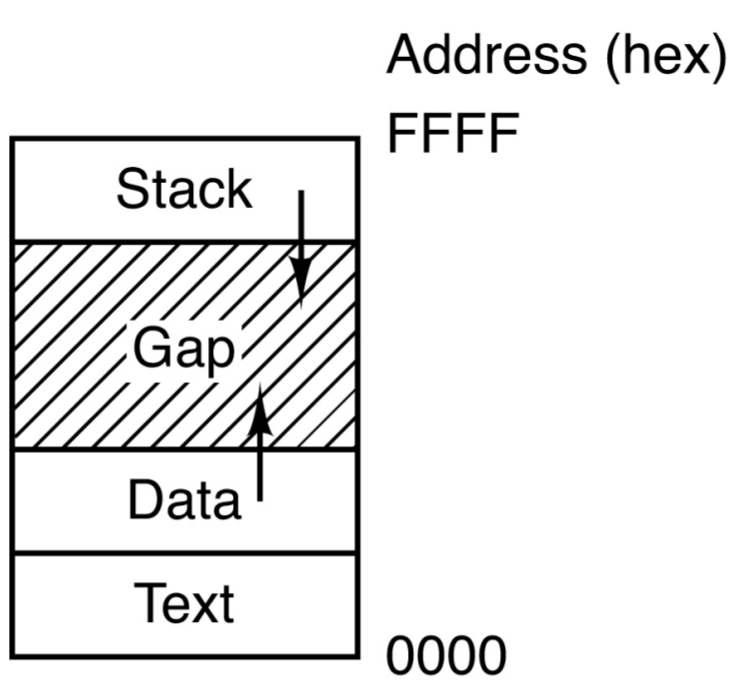
\includegraphics[width=0.2\textwidth]{AddressSpaceLayout}\end{figure}
\end{items}

\paragraph{OS Concepts --- Threads}
\begin{items}
	\item each progress: \( \geq 1 \) threads (representing execution states)
	\item IP stores currently executed instruction (address in \code{text} section)
	\item SP register stores address of stack top \\* (\( > 1 \) threads \( \to \) multiple stacks!)
	\item PSW contains flags about execution history \\* (e.g. last calculation was 0 \( \to \) used in following jump instruction)
	\item more general purpose registers, floating point registers,...
\end{items}
\begin{figure}[H]\centering\label{Threads}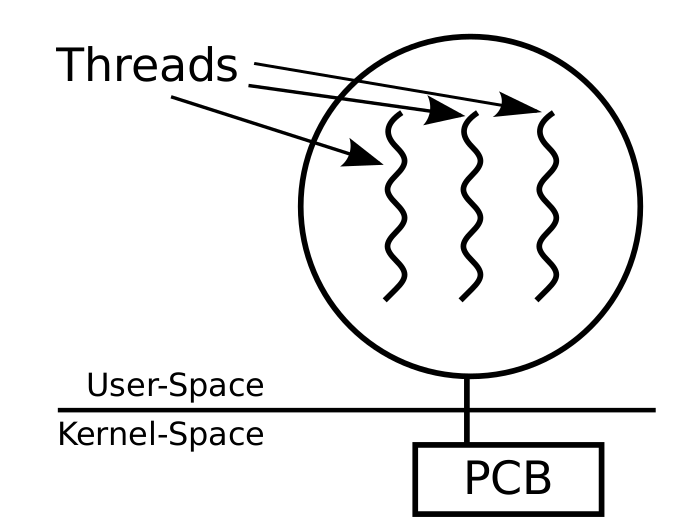
\includegraphics[width=0.2\textwidth]{Threads}\end{figure}

\paragraph{OS Concepts --- Policies vs. Mechanisms}
\begin{items}
	\item separation useful when designing OS
	\item \textbf{Mechanism}: implementation of what is done \\* (e.g. commands to put a HDD into standby mode)
	\item \textbf{Policy}: rules which decide when what is done and how much \\* (e.g. how often, how many resources are used,...)
	\item \( \to \) \emph{mechanisms can be reused even when policy changes}
\end{items}

\paragraph{OS Concepts --- Scheduling}
\begin{items}
	\item multiple processes/threads available \( \leadsto \) OS needs to switch between them (for multitasking)
	\item \emph{scheduler} decides which job to run next (policy)
	\item \emph{dispatcher} performs task-switching (mechanism)
	\item schedulers try to \\*
		- provide fairness \\*
		- while meeting goals \\*
		- and adhering to priorities
\end{items}
\begin{figure}[H]\centering\label{Scheduling}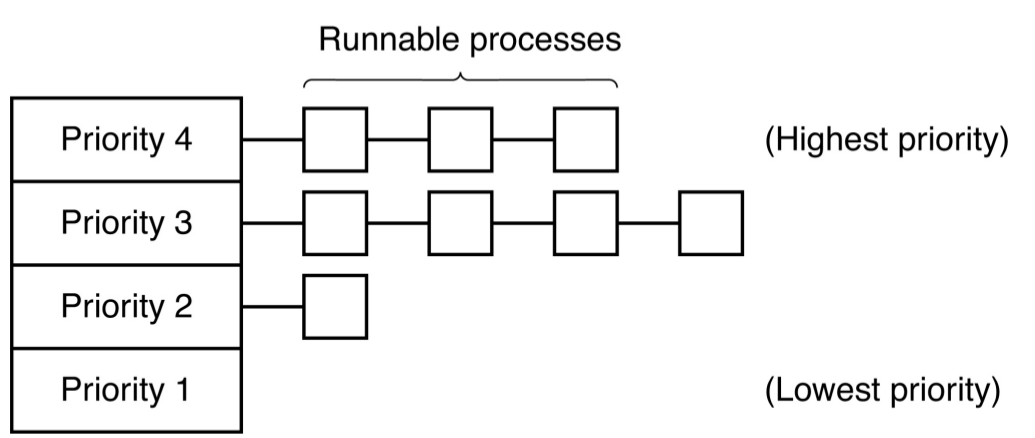
\includegraphics[width=0.33\textwidth]{Scheduling}\end{figure}

\paragraph{OS Concepts --- Files}
\begin{items}
	\item OS hides peculiarities of disks,...
	\item programmer uses device-independent \emph{files}/\emph{directories} for persistent storage
	\item \textbf{Files}: associate \emph{file name} and \emph{offset} with bytes
	\item \textbf{Directories}: associate \emph{directory names} with directory names or file names
	\item \textbf{File System}: ordered block collection \\*
		- main task: translate (dir name + file name + offset) to block \\*
		- programmer uses file system operations to operate on files \\* \phantom{-} (\code{open}, \code{read}, \code{seek})
	\item processes can communicate directly through special \emph{named pipe} file (used with same operations as any other file)
\end{items}

\paragraph{OS Concepts --- Directory Tree}
\begin{items}
	\item directories form \emph{directory tree}/\emph{file hierarchy} \\*
		\( \to \) structure data
	\item \emph{root directory}: topmost directory in tree
	\item files specified by providing \emph{path name} to file
\end{items}

\paragraph{OS Concepts --- Mounting}
\begin{items}
	\item Unix: common to orchestrate multiple file systems in single file hierarchy
	\item file systems can be \emph{mounted} on directory
	\item Win: manage multiple directory hierarchies with drive letters
		\\*
		(e.g. \code{C:\\Users})
\end{items}

\paragraph{OS Concepts --- Storage Management}
\begin{items}
	\item OS provides uniform view of information storage to file systems \\*
		- \emph{drivers} hide specific hardware devices \\* \phantom{-} \( \to \) hides device peculiarities \\*
		- general interface abstracts physical properties to logical units \\* \phantom{-} \( \to \) block
	\item OS increases I/O performance: \\*
		- \textbf{Buffering}: Store data temporarily while transferred \\*
		- \textbf{Caching}: Store data parts in faster storage \\*
		- \textbf{Spooling}: Overlap one job's output with other job's input
\end{items}

\begin{summary}
	\begin{items}
		\item OS provides abstractions for and protection between applications
		\item kernel does not always run --- certain events invoke kernel \\*
			$ - $ \emph{syscall}: process asks kernel for service \\*
			$ - $ \emph{interrupt}: device sends signal that OS has to handle \\*
			$ - $ \emph{exception}: CPU encounters unusual situation
		\item processes encapsulate resources needed to run program in OS \\*
			$ - $ \emph{threads}: represent different execution states of process \\*
			$ - $ \emph{address space}: all memory process can name \\*
			$ - $ \emph{resources}: allocated resources, e.g., open files
		\item scheduler decides which process to run next when multi-tasking
		\item virtual memory implements address spaces, provides protection between processes
	\end{items}
\end{summary}